\chapter{Mechanical Equilibrium}

In this chapter, we will study the mechanical equilibrium of objects. We often consider mechanical problems in the context of \emph{point objects}, in the case of a dimensionless point, there cannot be any turning moment and zero resultant force suffices for equilibrium. For \emph{rigid bodies}, any force many produce a turning effect called a \emph{moment}.

It follows then, that rigid bodies must satisfy another condition to stay in equilibrium...

\subsection{Moment of force}

\begin{ilight}
	The \keypoint{moment}\index{moment} of a force, is defined as the product of the force and the perpendicular distance from the pivot to the line of action. The word \keypoint{torque}\index{torque} is often used instead of moment, especially when we're \cancel{torquing} talking about the dynamic rotation of a motor and a change in angular momentum, rather than a statics problem. It's convenient to use $\tau$ as shorthand for moment: \begin{empheq}[box=\tcbhighmath]{equation*}{\tau = Fd_\perp} \end{empheq}
\end{ilight}

\begin{marginfigure}
	\centering
	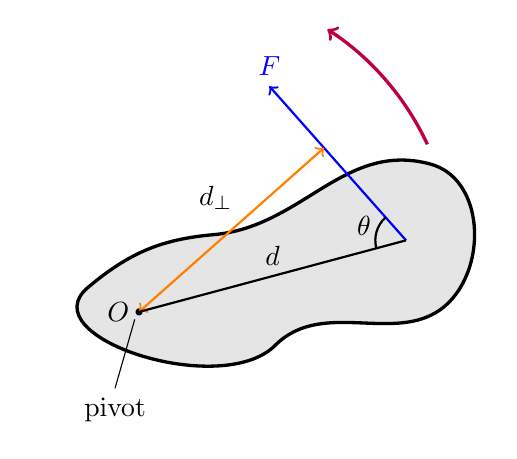
\begin{tikzpicture}[scale=0.78,rotate=15]
	\draw[fill=gray!20,very thick] (-3.2,0.4) to [out=25,in=170] (-1,0.7) to [out=-10,in=150] (2.7,0.9) to [out=-30,in=35] (2.5,-1.3) to [out=215,in=30] (-0.5,-1.3) to [out=210,in=205] (-3.2,0.4);
	\draw[thick,blue,->] (2,-.2) --++ (-1.5,3) node[above]{$F$};
	\draw[fill] (-2.5,-.2) circle (0.05) node[left]{$O$};
	\draw (-2.6,-.3) --++ (-.6,-1) node[below]{pivot};
	\draw[thick,orange,<->] (-2.5,-.2) --++ (26.565:4.025) node[pos=0.56,above left,black]{$d_\perp$};
	\draw[thick] (-2.5,-.2) -- (2,-.2) node[midway,above]{$d$};
	\draw[thick] (1.5,-.2) arc(180:116.565:.5);
	\node at (1.4,0.2) {$\theta$};
	\draw[very thick,purple,->] (24:3) arc(10:42:4.5);
	\end{tikzpicture}
 \caption{Moment of a shape}
 \label{fig:moment}
\end{marginfigure}

The unit of torque\sidenote[][-10cm]{You'll not learn about angular momentum unless you take the sports science option} or moment is the Newton-meter : $[\tau] = \text{N m}$\\

The critical part of working out the moment of a force is that the displacement from the axis of rotation and the force are perpendicular. This means that if you have an object like \ref{fig:moment} then you will need to resolve \emph{either} the force \emph{or} the displacement. Which one you choose resolve is immaterial, so you might as well use whichever is most convenient!\\
\example{In the diagram, if we resolve the displacement; $$d_\perp = d\sin\theta$$ the moment of this force is: $$\tau = Fd\sin\theta$$\\
If we resolve the force: $$F_\perp = F\sin\theta$$ so moment of this force is: $$\tau = F\sin\theta d$$}

The moment of a force is treated\footnote{\piste Rigorously speaking, moment is a \emph{pseudovector}, which means that it does not transform quite like a normal vector although it does have a direction. In particular, if an object acted by a force is reflected across a plane, the moment of this force would not be reflected. Instead, it would be reflected and \emph{reversed} as a vector quantity}
\footnote[][]{\piste Using vector notation, moment of a force can be defined as a \emph{cross product}: $\overrightarrow{\tau} = \overrightarrow{r}\times\overrightarrow{F}$, where $\overrightarrow{r}$ is the position vector from the pivot to the point at which the force is applied.}
it can act in \emph{clockwise} or \emph{anti-clockwise} direction. 

The moment of a force produces turning effects,\footnote{Moment is like the rotational counterpart of a force: force changes the state of translational motion, moment changes the state of rotation.} if there exists a non-zero moment, the object will have clockwise or anti-clockwise \emph{angular acceleration}.\\
\titem Note that moment of a force depends on choice of pivot location. The moment of the same force with respect to different points can be very different. We often use this trick in questions to reduce the difficulty of the problem or the number of calculations required.

\subsection{Torque of couple}\label{ch:torque-of-couple}

Let's take a pair of equal but opposite forces acting at different positions on the same object, as in the figure \ref{fig:torquecouple}.

\begin{marginfigure}
	\centering
	\vspace*{-8pt}
	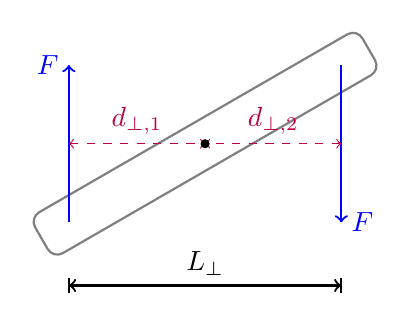
\begin{tikzpicture}
	\draw[thick,gray, rotate=30, rounded corners] (-2.4,-.3) rectangle (2.4,.3);
	\draw[thick,blue,->] (-1.73,-1) -- ++(0,2) node[left]{$F$};
	\draw[thick,blue,->] (1.73,1) -- ++(0,-2) node[right]{$F$};
	\draw[dashed,<->,purple] (-1.73,0) -- (0,0) node[midway,above]{$d_{\perp,1}$};
	\draw[dashed,<->,purple] (1.73,0) -- (0,0) node[midway,above]{$d_{\perp,2}$};
	\draw[fill] (0,0) circle(0.05);
	\draw[thick,<->] (-1.73,-1.8) -- (1.73,-1.8) node[midway,above]{$L_\perp$};
	\draw[thick] (-1.73,-1.9) -- (-1.73,-1.7) (1.73,-1.9) -- (1.73,-1.7);
	\end{tikzpicture}
	\vspace*{-16pt}
 \label{fig:torquecouple}
\end{marginfigure}

The two forces produce moments in the same direction, but because they have equal magnitudes and opposite directions, they produce no translational acceleration. The combined effect is called the torque of a couple. The resultant torque due to the couple is:

	$$ \tau = Fd_{\perp,1} + Fd_{\perp,2} = 2F(d_{\perp,1} + d_{\perp,2}) $$

$d_{\perp,1} + d_{\perp,2}$ is perpendicular distance $L_\perp$ between the pair, so:

$$ \tcbhighmath{\tau = F L_\perp} $$

\begin{ilight}
	\keypoint{Torque of a couple} can be therefore defined as the product of one force in the couple and the perpendicular distance between the pair
\end{ilight}
Note that: the torque of couple does not depend on choice of pivot. For same force pair, resultant moment is constant about any point.



\subsection{Moment of weight}

If you recall that weight is a force of gravity which is actually experienced by \emph{all} parts of the object, then you will realise  we need to sum up torques on each part of this object. This this brings a problem since the displacement of every part of the object will be different, fortunately, this calculation can be simplified using the idea of centre of gravity.

\begin{ilight}
	\keypoint{centre of gravity} is a point at which the entire weight of an object is considered to act\index{centre of gravity}
\end{ilight}

There is a similar concept called the centre of mass;

\keypoint{centre of mass} is the average position of all the mass that makes up the object.

Near the surface of the earth, mass and weight are directly proportional to each other so centre of mass is interchangeable with centre of gravity if we stay on earth\footnote{\piste You might like to explore this idea a bit - when and where would they be in a different part of a body?}.

For a regularly-shaped uniform object, the centre of gravity/mass is its geometrical centre, If an object is hung freely, centre of gravity/mass is vertically below the point of suspension, otherwise weight would produce a non-zero torque about the point of suspension, causing the object to rotate until torque becomes zero:

\begin{figure*}[ht]
	\centering
	\begin{minipage}[b]{0.45\textwidth}
		\centering
		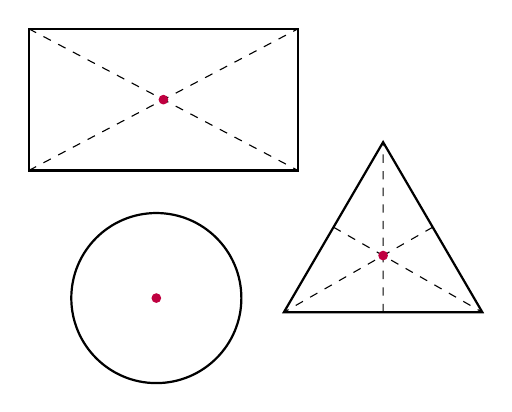
\begin{tikzpicture}[scale=0.9]
		% triangle
		\draw[thick] (-1.4,0) -- (0,2.4) -- (1.4,0) --cycle;
		\draw[dashed] (0,0) -- (0,2.4) (0.7,1.2) -- (-1.4,0) (-0.7,1.2) -- (1.4,0);
		\draw[purple,fill] (0,0.8) circle (0.06);
		% rectangle
		\draw[thick] (-5,2) rectangle (-1.2,4);
		\draw[dashed] (-5,2) -- (-1.2,4) (-5,4) -- (-1.2,2);
		\draw[purple,fill] (-3.1,3) circle (0.06);	
		% circle
		\draw[thick] (-3.2,0.2) circle(1.2);
		\draw[purple,fill] (-3.2,0.2) circle (0.06);		
		\end{tikzpicture}
	centre of mass of uniform lamina
		
		is at the geometrical centre
	\end{minipage}\hfil
	\begin{minipage}[b]{0.45\textwidth}
		\centering
		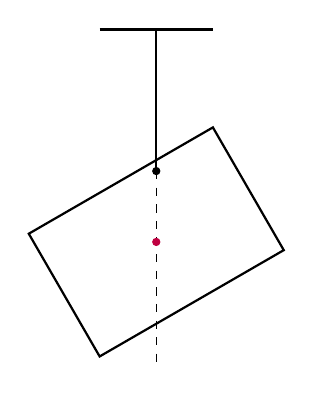
\begin{tikzpicture}[scale=0.9]
		\draw[thick,rotate=30] (-1.5,-1) rectangle (1.5,1);
		\draw[fill] (0,1) circle (0.05);
		\draw[thick] (0,1) -- (0,3);
		\draw[very thick] (-0.8,3) -- (0.8,3);
		\draw[dashed] (0,1) -- (0,-1.8);
		\draw[purple, fill] (0,0) circle (0.05);
		\end{tikzpicture}
		
		centre of mass is vertically below
		
		the point of suspension
	\end{minipage}
\end{figure*}

A simple, practical way to find the centre of gravity/mass of an object is to suspended it from several positions. Each time we draw a vertical \emph{plumb-line} through the point of suspension. The centre of mass/gravity lies where the lines intersect.
\section{Stability}

By using the idea of torque, we can easily understand how, or why some items are stable, and others less-so. When an object is sat on a level surface, undisturbed, the resultnt forces must pass through the centre of mass, resulting in no torque:
% BLOCK - metastable
\def\H{3.1} % block height
\def\W{1.4} % block width
\def\R{sqrt(\W^2+\H^2)/2} % block half-diagonal
\def\D{0.25} % ground depth
\def\ang{atan(\H/\W)} % angle diagonal ccw
\def\angcw{atan2(\H,-\W)} % angle diagonal cw

\begin{figure}[ht]
\centering
\begin{tikzpicture}[scale=1.5]
  \coordinate (O) at (0,0);
  \coordinate (CM) at (0,\H/2);
  \coordinate (BL) at (-\W/2,0); % bottom left corner
  \coordinate (BR) at (\W/2,0); % bottom right corner
  \coordinate (TR) at (\W/2,0); % top right corner
  \draw[ground] (-0.8*\W,0) rectangle (1.4*\W,-\D);
  \draw[thick] (-0.8*\W,0) -- (1.4*\W,0);
  \draw[mass] (-\W/2,0) rectangle++ (\W,\H);
  \node[left] at (-\W/2,\H/2) {$W$};
  \node[above] at (0,\H) {$H$};
  \draw[CM] (CM) circle(0.06*\W);
  \draw[dashed] (BR) -- (CM) --++ ({\angcw}:0.2*\W);
  \draw[dashed] (BR)++(130:{\R}) arc(130:35:{\R});
  \draw pic[myarr,"$\theta$"scale=0.9,draw,angle radius=18,angle eccentricity=1.35] {angle=TR--BR--CM};
  \draw[force] (CM) --++ (0,-0.24*\H) node[midway,below=2,left=-.1] {$m\vb{g}$};
  \draw[force] (O) --++ (0,0.24*\H) node[midway,left=-.1] {$\vb{F}_\mathrm{N}$};
  \node[mypurple,above right=.1] at (BR) {$\vb*\tau=0$};
  %\draw[->] (F)++(42:1.9*\L) arc(70:0:0.5*\L) node[midway,above right=-2] {$\alpha$};
  \draw[rvec] (BR) -- (CM) node[below,right] {$\vb{r}$};
  \draw[rvec] (BR) -- (O) node[midway,above] {$\vb{r}_\mathrm{t}$};
  %\draw[rvec] (BR) -- (O) node[midway,right=2,below=-1.5] {\contour{white}{$\vb{r}_\mathrm{t}$}};
  \fill[blue!50!black] (BR) circle(0.03*\W);
\end{tikzpicture}
\end{figure}
As soon as the block is disturbed from this position, there will be a resultant torque. If the torque produced causes the block to return to it's origional position we would say the object is \emph{stable}. 
\begin{marginfigure}
\centering
% BLOCK - torque
\begin{tikzpicture}[scale=1.5]
  \def\ang{11}
  \coordinate (CM) at ({\angcw-\ang}:{\R});
  \coordinate (BR) at (0,0); % bottom right corner
  \coordinate (BL) at ({180-\ang}:\W); % bottom left corner
  \coordinate (TR) at ({\ang}:\W); % bottom left corner
  \coordinate (T) at ({\angcw-\ang-8}:{1.15*\R}); % torque 
  \draw[ground] (-1.3*\W,0) coordinate (L) rectangle (0.9*\W,-\D);
  \draw[thick] (-1.3*\W,0) -- (0.9*\W,0);
  \draw[mass,rotate around=({-\ang}:(BR))]
    (-\W,0) rectangle++ (\W,\H);
  \draw[CM] (CM) circle(0.06*\W);
  \draw[dashed] (BR) --++ (0,{1.6*\R});
  \draw[dashed] (BR)++(120:{\R}) arc(120:40:{\R});
  \draw[force] (CM) --++ (0,-0.24*\H) node[midway,below=2,left=-1] {$m\vb{g}$};
  \draw[force] (BR) --++ (0,0.24*\H) node[below right=0] {$\vb{F}_\mathrm{N}$};
  \pic[scale=1] at (T) {Tin};
  \node[mypurple,above=1] at (T) {$\vb*\tau$};
  \draw pic[myarr,draw,angle radius=35,angle eccentricity=1.1] {angle=BL--BR--L};
  \draw[rvec] (BR) -- (CM) node[midway,below left=-2] {$\vb{r}$};
  \draw[->] (110:1.1*\H) arc(110:148:0.4*\H) node[above left=-1] {$\alpha$};
  \fill[blue!50!black] (BR) circle(0.03*\W);
\end{tikzpicture}
\end{marginfigure}
As you can see - there can be more than one stable position for most shapes;\footnote{except the Gombok, which is only stable in one orientation}:


\begin{marginfigure}
% BLOCK - plot
\centering
\begin{tikzpicture}
  \def\xmax{3.4}
  \def\ymax{2.8}
  \def\angms{25}            % unstable angle
  \def\angus{atan(tan(\angms))} % unstable angle
  \def\angne{60}            % non-equilibrium
  \def\A{2.0}               % amplitude / yscale
  \def\yW{\A*sin(\angms)}   % y position phi =  0
  \def\yH{\A*cos(\angms)}   % y position phi = 90
  \def\xH{0.7*\xmax}        % x position phi = 90
  \def\xi{(90-\angms)/\om}  % x position unstable
  \def\om{(90/(\xH))}
  \def\h{0.12*\xmax} % height mini block
  \def\w{\h*tan(\angus)} % width mini block
  \coordinate (O) at (0,0);
  \coordinate (P-2) at ({(\angus-90)/\om},0.014);
  \coordinate (P-1) at ({(\angne-90)/\om},0.013);
  \coordinate (P+1) at ({(90-\angne)/\om},0.018);
  \coordinate (P+2) at ({(90-\angus)/\om},0.018);
  
  % MASS BLOCKS
  \begin{scope}[opacity=0.5]
    \draw[mass,rounded corners=0.9]
      ({-\xH-\w/2},0.018) rectangle++ ({\w},\h) % phi = -90
      (-\h/2,0.018) rectangle++ (\h,{\w})       % phi = 0
      ({\xH-\w/2},0.018) rectangle++ ({\w},\h); % phi = +90
    \draw[mass,rotate around={{\angus}:(P-2)}]
      (P-2) rectangle++ ({\w},\h);
    \draw[mass,rotate around={{\angne}:(P-1)}]
      (P-1) rectangle++ ({\w},\h);
    \draw[mass,rotate around={{-\angne}:(P+1)}]
      (P+1) rectangle++ (-{\w},\h);
    \draw[mass,rotate around={{-\angus}:(P+2)}]
      (P+2) rectangle++ (-{\w},\h);
    \draw[very thin]
      ({\xH+\w/2+0.3*\h},0.018) arc(0:90:0.3*\h) node[pos=0.5,above right,scale=0.5] {$\phi$}
      (P+1)++(-5:0.50*\h) arc(-5:{90-\angne}:0.50*\h) node[pos=0.7,right,scale=0.5] {$\phi$}
      (P+2)++(-5:0.30*\h) arc(-5:{90-\angus}:0.30*\h) node[pos=0.5,above right,scale=0.5] {$\phi$};
    \draw[very thin,mydashed]
      (P-2) --++ (0,1.5*\h)
      (P-1) --++ (0,0.8*\h)
      (P+1) --++ (0,1.2*\h)
      (P+2) --++ (0,1.5*\h);
  \end{scope}
  \fill[blue!50!black!50]
    ({-\xH-\w/2},\h+0.015) circle (0.03)
    (-\h/2,0.015) circle (0.03)
    (P-2)++({90+\angus}:\h) circle (0.03)
    (P-1)++({90+\angne}:\h) circle (0.03)
    (P+1) circle (0.03)
    (P+2) circle (0.03)
    ({\xH+\w/2},0.015) circle (0.03);
  
  % PLOT
  \draw[->,thick] (0,-0.1*\ymax) -- (0,1.05*\ymax) node[below=3,left] {$U=mgh$};
  \draw[->,thick] (-1.05*\xmax,0) -- (1.05*\xmax,0) node[below left] {$\phi$}; %$[\si{\degree}]$ %\theta
  \tick{-\xH,0}{90} node[below,scale=0.9] {$-90^{\text{o}}$};
  \tick{\xH,0}{90} node[below,scale=0.9] {$90^{\text{o}}$};
  \node[below,below left,scale=0.9] at (O) {$0^{\text{o}}$};
  \draw[dashed] (-\xH,0) --++ (0,1.1*\A);
  \draw[dashed] (\xH,0) --++ (0,1.1*\A);
  \tick{0,{\yH}}{0} node[right,above left,scale=0.9] {$mgH/2$};
  \tick{0,{\yW}}{0} node[right,below left,scale=0.9] {$mgW/2$};
  \draw[dashed] (-1.2*\xH,{\yH}) -- (1.24*\xH,{\yH});
  \draw[dashed] (-1.2*\xH,{\yW}) -- (1.24*\xH,{\yW});
  \draw[very thick,orange!80!black,samples=100,smooth,variable=\t]
    plot[domain=-\xmax:-\xH](\t,{\A*sin(\om*abs(\t)-\angms)}) --
    plot[domain=-\xH:0](\t,{\A*sin(\om*abs(\t)+\angms)}) --
    plot[domain=0:\xH](\t,{\A*sin(\om*\t+\angms)}) --
    plot[domain=\xH:\xmax](\t,{\A*sin(\om*\t-\angms)}); %node[right] {$x$}
    
  % CENTER OF MASS
  \draw[CM] (-\xH,{\yH+0.1}) circle(0.08) node[below=1,scale=0.85,fill=white,inner sep=1] {metastable};
  \draw[CM] (\xH,{\yH+0.1}) circle(0.08) node[below=1,scale=0.85,fill=white,inner sep=1] {metastable};
  \draw[CM] ({(90-\angms)/\om},{\A+0.1}) circle(0.08) node[above=.5,scale=0.85] {unstable};
  \draw[CM] ({(\angms-90)/\om},{\A+0.1}) circle(0.08) node[above=.5,scale=0.85] {unstable};
  \draw[CM] (0,{\yW+0.1}) circle(0.08) node[below=.5,scale=0.85] {stable};
  
\end{tikzpicture}
\end{marginfigure}


If we apply these ideas to the real world we can use them to understand that one of the more impressive looking tricks of the circus can be brought into the hands of everyone. 
Consider a tightrope walker:
% TIGHT ROPE arms
\def\L{3.2}   % length
\def\T{0.08}  % plank thickness
\def\H{2.2}   % human height
\def\CM{0.06} % CM radius
\begin{marginfigure}
\centering
   \begin{tikzpicture}
  \coordinate (O) at (0,0);
  \draw[rope] (O) circle (0.08);
  \draw[thick] (0,\H) circle(0.3) coordinate (H);
  \draw[thick] (H)++(-90:0.3) coordinate (N) to[out=-92,in=92]++ (0,-0.40*\H) coordinate (P);
  \draw[limb] (N)++(-120:0.03) to[out=-120,in=30]++ (-0.27*\H,-0.3*\H); % right arm
  \draw[limb] (N)++(-60:0.03) to[out=-60,in=140]++ (0.27*\H,-0.3*\H);   % left arm
  \draw[limb] (P) to[out=-95,in=95] (96:0.1); % right leg
  \draw[limb] (P) to[out=-85,in=88] (84:0.1); % left leg
  \draw[CM] (0,0.54*\H) circle(\CM) node[below right=0,scale=0.8] {CM};
\end{tikzpicture}
    \caption{Walking on a tight-rope unaided.}
    \label{fig:tightrope}
\end{marginfigure}

We can see that the Centre of Mass is substantially higher than the contact point and the situation is unstable. The artist has to be quite active in maintaining their CoM above the contact point - it's hard work!

One of the tricks that you can use however is a long pole to assist balance. Not only does this give you a mass that's easy to move around but it lowers the center of mass:
\begin{marginfigure}
% TIGHT ROPE - stick
\centering
\begin{tikzpicture}
  \coordinate (O) at (0,0);
  \draw[rope] (O) circle (0.08);
  \draw[thick] (0,\H) circle(0.3) coordinate (H);
  \draw[thick] (H)++(-90:0.3) coordinate (N) to[out=-91,in=92]++ (0,-0.40*\H) coordinate (P);
  \draw[limb] (P) to[out=-95,in=95] (96:0.1); % left leg
  \draw[limb] (P) to[out=-85,in=88] (84:0.1); % right leg
  \draw[myred,line width=1.5,line cap=round]
    (-\H,0.1*\H) to[out=40,in=180] (0,0.47*\H) to[out=0,in=140] (\H,0.1*\H);
  \draw[limb] (N)++(-95:0.03) to[out=-120,in=80]++ (-0.19*\H,-0.4*\H); % right arm
  \draw[limb] (N)++(-85:0.03) to[out=-60,in=100]++ (0.19*\H,-0.4*\H);   % left arm
  \draw[CM] (0,0.3*\H) circle(\CM) node[below right=0,scale=0.8] {CM};
\end{tikzpicture}
\end{marginfigure}
This might be clearer if we picture the kind of balance support given to beginners: 
\begin{marginfigure}
% TIGHT ROPE - weights
\begin{tikzpicture}
  \def\L{1.2}  % handle length
  \def\w{0.3}  % mass width
  \def\h{0.45} % mass height
  \def\r{0.02} % rope radius
  \coordinate (O) at (0,0);
  \coordinate (SL) at (-\L/2,0.42*\H); % stick left
  \coordinate (SR) at ( \L/2,0.42*\H); % stick right
  \coordinate (ML) at (-\L/2,-0.2*\H); % mass left
  \coordinate (MR) at ( \L/2,-0.2*\H); % mass right
  \draw[rope] (O) circle (0.08);
  \draw[thick] (0,\H) circle(0.3) coordinate (H);
  \draw[thick] (H)++(-90:0.3) coordinate (N) to[out=-91,in=92]++ (0,-0.40*\H) coordinate (P);
  \draw[limb] (P) to[out=-95,in=95] (96:0.1); % left leg
  \draw[limb] (P) to[out=-85,in=88] (84:0.1); % right leg
  \draw[myred,line width=1.5,line cap=round] (SL)++(-0.05,0) -- (SR) --++ (0.05,0);
  \draw[limb] (N)++(-95:0.03) to[out=-120,in=85]++ (-0.14*\H,-0.44*\H); % right arm
  \draw[limb] (N)++(-85:0.03) to[out=-60,in=95]++ (0.14*\H,-0.44*\H);   % left arm
  \draw[CM] (0,-0.15*\H) circle(\CM) node[below=.5,scale=0.8] {CM};
  \draw[rope] (SL)++(-\r,0.02) arc(180:0:\r) -- ($(ML)+(\r,0)$) --++ (-2*\r,0) -- cycle;
  \draw[rope] (SR)++(-\r,0.02) arc(180:0:\r) -- ($(MR)+(\r,0)$) --++ (-2*\r,0) -- cycle;
  \draw[mass] (ML)++(-\w/2,-\h) rectangle++ (\w,\h);
  \draw[mass] (MR)++(-\w/2,-\h) rectangle++ (\w,\h);
\end{tikzpicture}
\end{marginfigure}


\begin{marginfigure}
	\vspace*{-8pt}
	\centering
	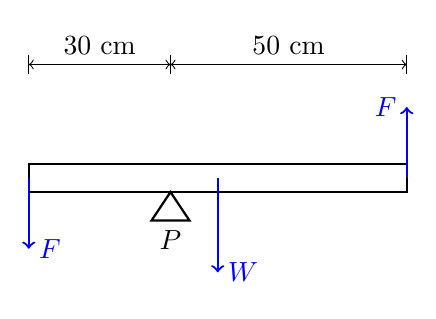
\begin{tikzpicture}[scale=0.6]
	\draw[thick] (-4,-.3) rectangle (4,.3);
	\draw[thick] (-1,-.3) --++ (.4,-.6) --++ (-.8,0) node[midway,below]{$P$} -- cycle;
	\draw[thick,blue,->] (0,0) -- (0,-2) node[right]{$W$};
	\draw[thick,blue,->] (4,0) --++ (0,1.5) node[left]{$F$};
	\draw[thick,blue,->] (-4,0) --++ (0,-1.5) node[right]{$F$};
	\draw[<->] (-4,2.4) -- (-1,2.4)node[midway,above]{30 cm};
	\draw[<->] (-1,2.4) -- (4,2.4)node[midway,above]{50 cm};
	\foreach \x in {-4,-1,4} \draw (\x,2.2) --++ (0,.4);
	\end{tikzpicture}
	\vspace*{-16pt}
\end{marginfigure}


\example{The diagram shows a uniform beam of weight $W=20 \text{ N}$ and length 80 cm pivoted at point $P$. $P$ is 30 cm from one end. Two equal but opposite forces of magnitude $F = 12 \text{ N}$ are acting at the two ends of the beam as shown. What is the resultant moment about point $P$?}

\begin{soln} Moment of weight: $\tau_w = W d_w = 20 \times \left(0.50-\frac{1}{2}\times0.80\right) = 2.0 \text{ N m} \quad$ (clockwise)

Torque of couple: $\tau_c = F L = 12 \times 0.80 = 9.6 \text{ N m} \quad$ (anti-clockwise)

Resultant moment: $\tau_\text{net} = \tau_c - \tau_W = 9.6 - 2.0 = 7.6 \text{ N m} \quad$ (anti-clockwise) \end{soln}

\subsection{Principle of moments}

If there is no turning effect for an object, the total moment of all forces must vanish:

\begin{ilight}
	For a rigid body in equilibrium, sum of all clockwise moments must be equal to the sum of anti-clockwise moments \emph{about any point}, this is called the \keypoint{principle of moments} \index{principle of moments}
\end{ilight}

IE.an object in equilibrium has no turning effect about any point so resultant moment is zero about any point.\\
\footnote{As long as there is no resultant force, then zero resultant moment about any particular point would imply zero resultant moment about any point.
	
Mathematically, let's take a collection of forces $\overrightarrow{F_1}, \overrightarrow{F_2}, \cdots, \overrightarrow{F_n}$ acting at positions $\overrightarrow{r_1}, \overrightarrow{r_2}, \cdots, \overrightarrow{r_n}$ on an object with respect to some fixed point $O$. Suppose their resultant moment vanishes, i.e., $\sum \overrightarrow{\tau_i} \equiv \sum\overrightarrow{r_i} \times \overrightarrow{F_i} =0$, and also their resultant force vanishes, i.e., $\sum \overrightarrow{F_i} = 0$. If we focus on a different point $O'$ with a relative displacement $\overrightarrow{R}$ to point $O'$, then taking moments about $O'$, we will have:
\begin{equation*}
	\sum \overrightarrow{\tau_i'} = \sum \overrightarrow{r_i'}\times\overrightarrow{F_i} = \sum (\overrightarrow{r_i}+\overrightarrow{R})\times\overrightarrow{F_i} = \sum \overrightarrow{r_i}\times\overrightarrow{F_i} + \overrightarrow{R} \times \sum\overrightarrow{F_i} = 0
\end{equation*}
which shows zero resultant moment about one point together with zero resultant force guarantee resultant moment must be zero about any point in space.}

\begin{marginfigure}
	\vspace*{-8pt}
	\centering
	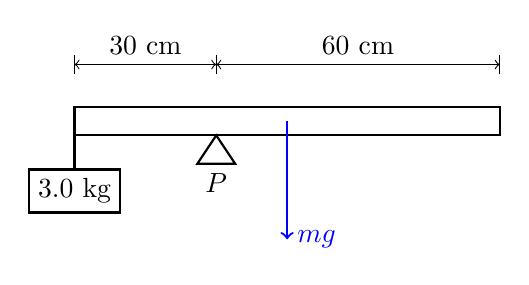
\begin{tikzpicture}[scale=0.6]
	\draw[thick] (-4.5,-.3) rectangle (4.5,.3);
	\draw[thick] (-1.5,-.3) --++ (.4,-.6) --++ (-.8,0) node[midway,below]{$P$} -- cycle;
	\draw[thick,blue,->] (0,0) -- (0,-2.5) node[right]{$mg$};
	\draw[<->] (-4.5,1.2) -- (-1.5,1.2)node[midway,above]{30 cm};
	\draw[<->] (-1.5,1.2) -- (4.5,1.2)node[midway,above]{60 cm};
	\foreach \x in {-4.5,-1.5,4.5} \draw (\x,1) --++ (0,.4);
	\draw[thick] (-4.5,0) --++ (0,-1) node[below, rectangle,draw]{3.0 kg};
	\end{tikzpicture}
	\vspace*{0pt}
\end{marginfigure}

\example{A uniform rod of length 90 cm is pivoted 30 cm from one end. It is balanced with a 3.0 kg load. Find the mass of the rod.}

\begin{soln}
    
 Take moments about $P$:
	
	$ 3.0 \times 9.81 \times 0.30 = m \times 9.81 \times \left(0.60-\frac{1}{2}\times0.90\right)$

so we find mass of rod: $m = 6.0 \text{ kg}$ 
\end{soln}


\example{A student balances a metre rule of mass 120 g supported on a fulcrum at the 40 cm mark. She then places a 20 g mass on the 70 cm mark and a 50 g mass on the 25 cm mark as shown. To balance the rule, what mass should she place on the 15 cm mark?}

\begin{figure}[ht]
	\centering
	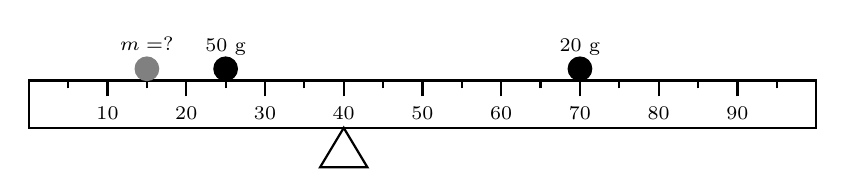
\begin{tikzpicture}[scale=1]
	\draw[thick] (-5,-.3) rectangle (5,.3);
	\foreach \x in {10,20,...,90} \draw[thick] (\x/10-5,.1) node[below]{{\scriptsize \x}} --++ (0,.2) ; 
	\foreach \x in {5,15,...,95} \draw[thick] (\x/10-5,.2) --++ (0,.1) ; 
	\draw[thick] (-1,-.3) --++ (.3,-.5) --++ (-.6,0) -- cycle;
	\draw[fill] (2,.45) circle (0.15);
	\node[above] at (2,.5) {{\scriptsize 20 g}};
	\draw[fill] (-2.5,.45) circle (0.15);
	\node[above] at (-2.5,.5) {{\scriptsize 50 g}};
	\draw[gray,fill] (-3.5,.45) circle (0.15);
	\node[above] at (-3.5,.56) {{\scriptsize $m=?$}};
	\end{tikzpicture}
\end{figure}

\begin{soln}
    
 Take moments about the support:
\begin{equation*}
	mg \times (40-15) + 0.050g\times(40-25) = \end{equation*}
 \begin{equation*}
     0.12g\times(50-40) + 0.020g\times(70-40) \RA m=42 \text{ g} 
\end{equation*}
\end{soln}

\example{A cylinder of weight 100 N and diameter 50 cm rests against point $P$ of a curb of height 10 cm. What is the minimum force required to cause the cylinder to roll to the left?}

\begin{marginfigure}
	\vspace*{-15pt}
	\centering
	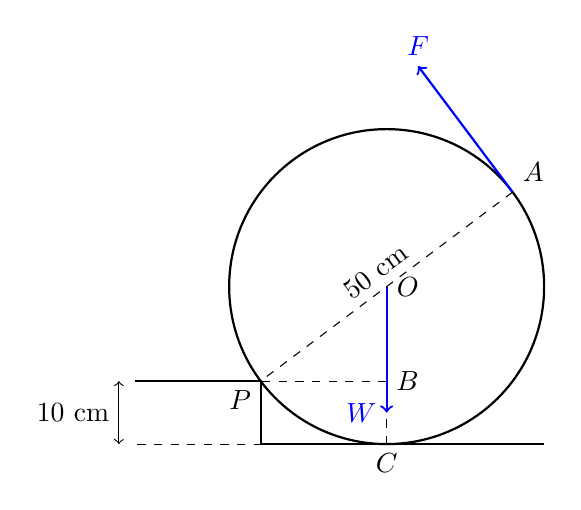
\begin{tikzpicture}[scale=0.4]
	\draw[thick] (0,0) circle (5) node[right]{$O$};
	\draw[thick] (-8,-3) -- (-4,-3) -- (-4,-5) --++ (9,0);
	\draw[thick,blue,->] (4,3) node[above right, black]{$A$} --++ (-3,4) node[above]{$F$};
	\draw[dashed] (4,3) -- (-4,-3) node[midway, above,rotate=36.87] {50 cm};
	\draw[dashed] (0,-3) node[right] {$B$}-- (-4,-3) node[below left] {$P$};
	\draw[dashed] (0,0) -- (0,-5) node[below] {$C$} -- (-8,-5);
	\draw[thick,blue,->] (0,0) -- (0,-4) node[left]{$W$};
	\draw[<->] (-8.5,-3) -- (-8.5,-5) node[midway, left] {10 cm};
	\end{tikzpicture}
	\vspace*{-0pt}
\end{marginfigure}


\begin{soln} To roll the cylinder, force applied must produce a torque no less than that of weight. The force is minimum if perpendicular displacement is greatest. 
Take moments about $P$ (see diagram):
	$ F_\tmin \times |PA| = W \times |PB| $


Note that $|PB| = \sqrt{|OP|^2 - |OB|^2}$, so
$|PB| = \sqrt{0.25^2 - (0.25-0.10)^2} = 0.20 \text{ m} $

Plug back into the equation above:
\begin{equation*}
	F_\tmin \times 0.50 = 100 \times 0.20 \RA F_\tmin = 40 \text{ N} 
\end{equation*}
\end{soln}

\subsection{Mechanical equilibrium}

Combining Newton's first law and principle of moments, we have the following statement:

\begin{ilight}
	For any mechanical system in equilibrium, two conditions must be satisfied:
	
	\begin{compactenum}
		\item[--] resultant force is zero in any direction: $\sum F = 0$
		
		\item[--] resultant moment is zero about any point: $\sum \tau = 0$
	\end{compactenum}
\end{ilight}

These two conditions allow for many problems to be solved.

\begin{marginfigure}
	\vspace*{-8pt}
	\centering
	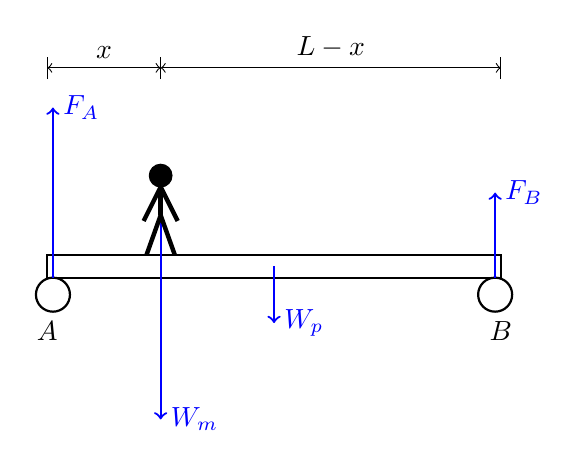
\begin{tikzpicture}[scale=0.72]
	\draw[thick] (-4,-.2) rectangle (4,.2);
	\draw[thick] (-3.9,-.5) circle(.3);
	\draw[thick] (3.9,-.5) circle(.3);
	\draw[thick,blue,->] (0,0) -- (0,-1) node[right]{$W_p$};
	\draw[thick,blue,->] (-2,0.8) --++ (0,-3.5) node[right]{$W_m$};
	\draw[thick,blue,->] (-3.9,-.2) --++ (0,3) node[right]{$F_A$};
	\draw[thick,blue,->] (3.9,-.2) --++ (0,1.5) node[right]{$F_B$};
	\draw[<->] (-4,3.5) -- (-2,3.5)node[midway,above]{$x$};
	\draw[<->] (-2,3.5) -- (4,3.5)node[midway,above]{$L-x$};
	\foreach \x in {-4,-2,4} \draw (\x,3.3) --++ (0,.4);
	\node[below] at (-4,-.8) {$A$};
	\node[below] at (4,-.8) {$B$};
	\draw[fill] (-2,1.6) circle(0.2);
	\draw[ultra thick] (-2,1.5) -- (-2,0.9);
	\draw[ultra thick] (-2,0.9) -- (-2.25,0.2) (-2,0.9) -- (-1.75,0.2);
	\draw[ultra thick] (-2.3,0.8) -- (-2,1.4) -- (-1.7,0.8);
	\end{tikzpicture}
	\vspace*{0pt}
\end{marginfigure}


\example{A uniform plank of weight 100 N and length $L=6.0 \text{ m}$ rests horizontally on two supports $A$ and $B$. A man of weight 800 N stands a distance of $x=1.5 \text{ m}$ from end $A$. Determine the forces acting at the two supports.}

\begin{soln} Take moments about $A$: $ W_m x + W_p \cdot\frac{L}{2} = F_B L$

{
	\centering

	
	$ 800 \times 1.5 + 100 \times 3.0 = F_B \times 6.0 \ra F_B = 250 \text{ N} $
	
}

Take moments about $B$: $ W_m (L-x) + W_p \frac{L}{2} = F_A L$

{
	\centering

	$ 800 \times 4.5 + 100 \times 3.0 = F_A \times 6.0 \ra F_B = 650 \text{ N} $
	
}

One can check that: $F_A + F_B = W_m + W_p$, there must be no resultant force in vertical direction \end{soln}


\begin{marginfigure}
	\vspace*{0pt}
	\centering
	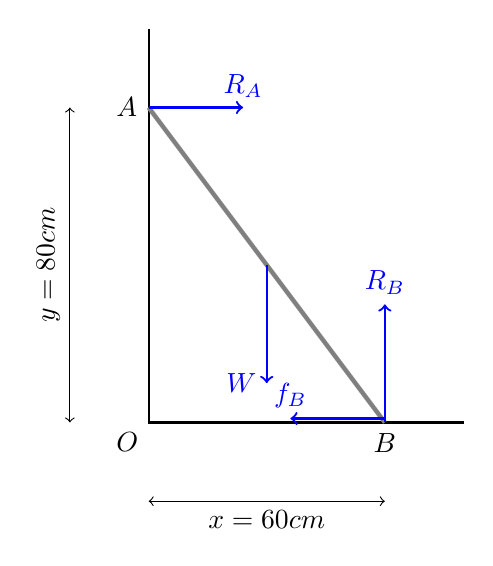
\begin{tikzpicture}[scale=1]
	\draw[thick] (0,5) -- (0,0) node[below left]{$O$} -- (4,0);
	\draw[ultra thick, gray] (0,4) node[left,black]{$A$} -- (3,0) node[below,black]{$B$};
	\draw[<->] (-1,0) -- (-1,4) node[above,midway,rotate=90]{$y=80\text{ cm}$};
	\draw[<->] (0,-1) -- (3,-1) node[below,midway]{$x=60\text{ cm}$};
	\draw[thick,blue,->] (0,4) --++ (1.2,0) node[above]{$R_A$};
	\draw[thick,blue,->] (3,0) --++ (0,1.5) node[above]{$R_B$};
	\draw[thick,blue,->] (3,0.05) --++ (-1.2,0) node[above]{$f_B$};
	\draw[thick,blue,->] (1.5,2) --++ (0,-1.5) node[left]{$W$};
	\end{tikzpicture}
	\vspace*{-16pt}
\end{marginfigure}


\example{A uniform ladder of weight 120 N rests on a rough ground against a smooth wall as shown. The dimensions are labelled on the diagram. (a) What is the contact force acting at $B$? (b) What is the contact force acting at $A$? (c) What is the frictional force at $B$?}


\begin{soln} Free-body diagram is drawn as shown

resolve vertically: $R_B = W \RA R_B = 120 \text{ N}$

take moments about $B$: $R_A y = W \frac{x}{2}$

{
	\centering
	
	$ R_A = \frac{120 \times 0.30}{0.80} = 45 \text{ N}$
	
}

resolve horizontally: $f_B = R_A \RA f_B = 45 \text{ N}$ 
\end{soln}
\begin{marginfigure}
	\vspace*{-12pt}
	\centering
	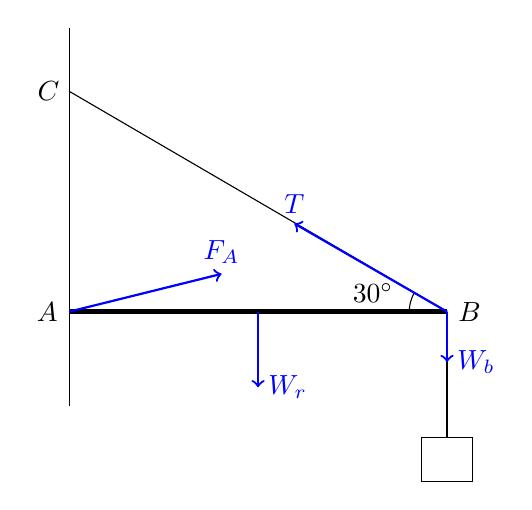
\begin{tikzpicture}[scale=0.8]
	\draw (0,-1.5) -- (0,4.5);
	\draw[ultra thick] (0,0) node[left]{$A$} -- (6,0) node[right]{$B$};
	\draw (6,0) -- (0,3.5) node[left]{$C$};
	\draw (5.4,0) arc(180:150:0.6);
	\node[left] at (5.3,0.3) {$30^\circ$};
	\draw (6,0) -- (6,-2);
	\draw (5.6,-2.7) rectangle (6.4,-2);
	\draw[thick,blue,->] (6,0) --++ (0,-0.8)node[right]{$W_b$};
	\draw[thick,blue,->] (3,0) --++ (0,-1.2)node[right]{$W_r$};
	\draw[thick,blue,->] (6,0) --++ (150:2.8)node[above]{$T$};
	\draw[thick,blue,->] (0,0) --++ (12.1*.2,3*.2)node[above]{$F_A$};
	\end{tikzpicture}
	\vspace*{-20pt}
\end{marginfigure}


\example{The diagram shows a uniform rod $AB$ of weight 60 N being held horizontally to a vertical wall by means of a light string. The string is attached to the rod at $B$, where a basket of weight 40 N is suspended. The other end of the string is fixed on the wall at $C$. The angle between the string and the rod is $30^\circ$. (a) Find the tension in the string. (b) Find the force acting on the rod at point $A$.}

\begin{soln} Take moments about $A$: $TL\sin\theta = W_b L + W_r  \frac{1}{2}L$

{
	\centering
	
	$ T \sin30^\circ = 40 + 60\times\frac{1}{2} \RA T=140 \text{ N} $
	
}

resolve horizontally: $F_{A,x} = T\cos\theta \RA F_{A_x}=140\cos30^\circ \approx 121 \text{ N}$

resolve vertically: $F_{A,y}+T\sin\theta = W_r + W_b \RA F_{A,y} = 60+40 - 140\sin30^\circ = 30 \text{ N} $

force at $A$: $F_A = \sqrt{F_{A,x}^2 + F_{A,y}^2} \RA F_A = \sqrt{121^2 + 30^2} \approx 125 \text{ N}$ \end{soln}


\subsection{Two forces in equilibrium}

The problem of two balanced forces is trivial

\begin{marginfigure}
	\vspace{-15pt}
	\begin{center}
		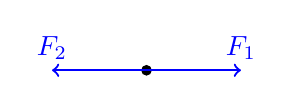
\begin{tikzpicture}[scale=0.6]
		\draw[fill] (0,0) circle(0.1);
		\draw[thick,blue,->] (0,0) -- (2,0) node[above]{$F_1$};
		\draw[thick,blue,->] (0,0) -- (-2,0) node[above]{$F_2$};
		\end{tikzpicture}
	\end{center}
	\vspace{-10pt}
\end{marginfigure}

Suppose two forces $F_1$ and $F_2$ are acting on an object in equilibrium

\begin{compactenum}
	\item[--] to have zero resultant force, $F_1$ and $F_2$ must be equal but opposite
	
	\item[--] to have zero resultant moment, $F_1$ and $F_2$ must act along same line
	
	otherwise they produce torque of couple that causes turning effects
\end{compactenum}


\subsection{Three forces in equilibrium}

\subsection{Force triangle}

When there are more than two forces, the situation becomes more complicated and we use \emph{vector diagrams} to solve the problems.

Suppose a set of forces $\overrightarrow{F_1}$, $\overrightarrow{F_2}$, $\cdots$, $\overrightarrow{F_n}$ are in equilibrium. If that's the case then no resultant force requires $\overrightarrow{F_1} + \overrightarrow{F_2} + \cdots + \overrightarrow{F_n} = 0$

Recall that resultant force is vector sum of all forces acting, and now this sum has to vanish, so if the force vectors are connected head to tail, they should form a closed $n$-polygon:

\begin{figure}[ht]
	\centering
	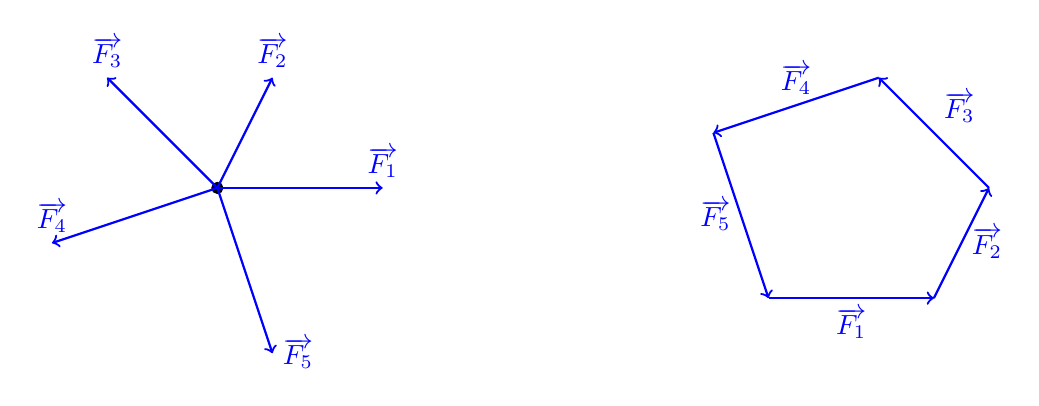
\begin{tikzpicture}[scale=0.7]
	\draw[fill] (0,0) circle(0.1);
	\draw[thick,blue,->] (0,0) -- (3,0) node[above]{$\overrightarrow{F_1}$};
	\draw[thick,blue,->] (0,0) -- (1,2) node[above]{$\overrightarrow{F_2}$};
	\draw[thick,blue,->] (0,0) -- (-2,2) node[above]{$\overrightarrow{F_3}$};
	\draw[thick,blue,->] (0,0) -- (-3,-1) node[above]{$\overrightarrow{F_4}$};
	\draw[thick,blue,->] (0,0) -- (1,-3) node[right]{$\overrightarrow{F_5}$};
	
	\node at (6,0) {\Huge{$\RA$}};
	
	\draw[thick,blue,->] (10,-2) -- ++(3,0) node[midway,below]{$\overrightarrow{F_1}$};
	\draw[thick,blue,->] (13,-2)-- ++(1,2) node[midway,right]{$\overrightarrow{F_2}$};
	\draw[thick,blue,->] (14,0)-- ++(-2,2) node[midway,above right]{$\overrightarrow{F_3}$};
	\draw[thick,blue,->] (12,2)-- ++(-3,-1) node[midway,above]{$\overrightarrow{F_4}$};
	\draw[thick,blue,->] (9,1) -- ++(1,-3) node[midway,left]{$\overrightarrow{F_5}$};
	\end{tikzpicture}
	\caption{an $n$-polygon formed by a set of $n$ balanced forces}\label{fig:force-polygon}
\end{figure}

In the case of three balanced forces, net force is zero means they should form a \keypoint{force triangle}. Any unknown forces can then be solved by cracking a geometric problem.

\begin{marginfigure}
	\vspace*{-16pt}
	\centering
	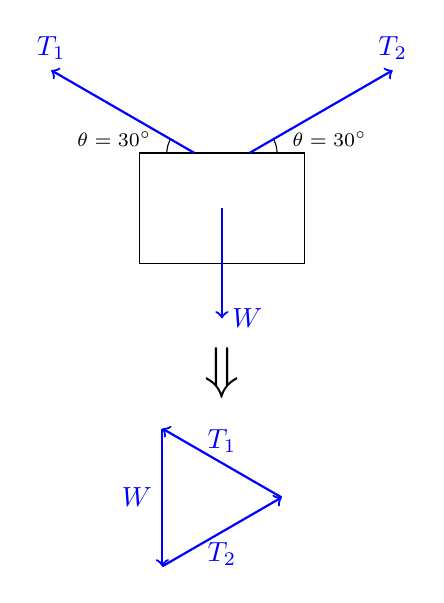
\begin{tikzpicture}[scale=0.7]
	\draw (-1.5,0) rectangle (1.5,-2);
	\draw[->,thick,blue] (0,-1) -- (0,-3) node[right]{$W$};
	\draw[->,thick,blue] (-0.5,0) -- ++(150:3) node[above]{$T_1$};
	\draw (-1,0) arc(180:150:0.5);
	\node[left] at (-1.1,0.25) {\scriptsize$\theta=30^\circ$};
	\draw (1,0) arc(0:30:0.5);
	\node[right] at (1.1,0.25) {\scriptsize$\theta=30^\circ$};
	\draw[->,thick,blue] (0.5,0) -- ++(30:3) node[above]{$T_2$};
	\node at (0,-4) {\huge{$\Downarrow$}};
	\draw[->,,thick,blue] (-1.0825,-5) -- ++(0,-2.5) node[midway,left]{$W$};
	\draw[->,,thick,blue] (-1.0825,-7.5) -- ++(30:2.5) node[midway,below]{$T_2$};
	\draw[<-,,thick,blue] (-1.0825,-5) -- ++(-30:2.5) node[midway,above]{$T_1$};
	\end{tikzpicture}
	\vspace*{-10pt}
\end{marginfigure}

\example{A painting of weight $W=20\text{ N}$ is supported by two strings as shown. Both strings form an angle $\theta=30^\circ$ to the horizontal. Find the tension in the strings.}



\begin{soln} By resolving forces, we have: 

{
	\centering
	
	$\Biggl\{\begin{array}{l}
	T_1 \cos\theta = T_2 \cos\theta\\
	T_1\sin\theta + T_2\sin\theta = W
	\end{array} $ 
	
}

we solve the equations to obtain:

{
	\centering
	
	$ T_1 = T_2  = \frac{W}{2\sin\theta} = \frac{20}{2\sin30^\circ}=20\text{ N} $
	
}


alternatively, we can construct the force triangle as shown

$T_1$, $T_2$ and $W$ form an equilateral triangle, so
\begin{equation*}
	T_1=T_2=W=20\text{ N} 
\end{equation*}
\end{soln}
\begin{marginfigure}
	\vspace*{-12pt}
	\centering
	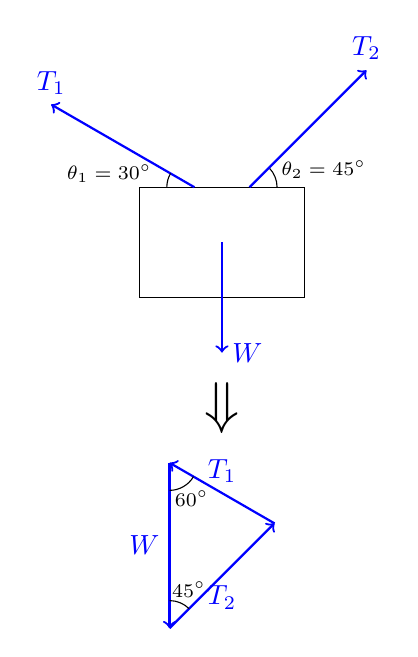
\begin{tikzpicture}[scale=0.7]
	\draw (-1.5,0) rectangle (1.5,-2);
	\draw[->,thick,blue] (0,-1) -- (0,-3) node[right]{$W$};
	\draw[->,thick,blue] (-0.5,0) -- ++(150:3) node[above]{$T_1$};
	\draw (-1,0) arc(180:150:0.5);
	\node[left] at (-1.1,0.25) {\scriptsize$\theta_1=30^\circ$};
	\draw (1,0) arc(0:45:0.5);
	\node[right] at (0.9,0.32) {\scriptsize$\theta_2=45^\circ$};
	\draw[->,thick,blue] (0.5,0) -- ++(45:3) node[above]{$T_2$};
	\node at (0,-4) {\huge{$\Downarrow$}};
	\draw[->,,thick,blue] (-.95,-5) -- ++(0,-3) node[midway,left]{$W$};
	\draw[->,,thick,blue] (-0.95,-8) -- ++(45:2.69) node[midway,below]{$T_2$};
	\draw[<-,,thick,blue] (-.95,-5) -- ++(-30:2.20) node[midway,above]{$T_1$};
	\draw (-0.95,-5.5) arc(-90:-30:0.5);
	\draw (-0.95,-7.5) arc(90:45:0.5);
	\node at (-0.55,-5.65) {{\scriptsize $60^\circ$}};
	\node at (-0.6,-7.3) {{\scriptsize $45^\circ$}};
	\end{tikzpicture}
	\vspace*{-18pt}
\end{marginfigure}

\example{The same painting of weight $W=20\text{ N}$ is supported by two strings at different angles $\theta_1=30^\circ$ and $\theta_2=45^\circ$ as shown. Find the forces in the two strings.}


\begin{soln} By resolving forces, we have: 

{
	\centering
	
	$ \left\{\begin{array}{l}
		T_1 \cos\theta_1 = T_2 \cos\theta_2\\
		T_1\sin\theta_1 + T_2\sin\theta_2 = W
	\end{array} \right.
	\RA
	\left\{\begin{array}{l}
	\frac{\sqrt{3}}{2}T_1 = \frac{\sqrt{2}}{2}T_2\\
	\frac{1}{2}T_1 + \frac{\sqrt{2}}{2}T_2 = 20
	\end{array} \right.
	$
	
}


solving this, we find: $T_1 \approx 14.6\text{ N}\, , \, T_2 \approx 17.9\text{ N} $

alternatively, we construct the force triangle as shown

$T_1$ and $T_2$  are related to $W$ by the the law of sine:

{
	\centering
	
	$\frac{W}{\sin75^\circ} = \frac{T_1}{\sin45^\circ} = \frac{T_2}{\sin60^\circ} $
	
}

from this we get the same result: $T_1 \approx 14.6\text{ N}\, , \, T_2 \approx 17.9\text{ N} $ \end{soln}



\subsection{Concurrent forces}

Tor three forces in equilibrium, they must produce zero resultant moment about any point.

\begin{marginfigure}
	\vspace*{-15pt}
	\centering
	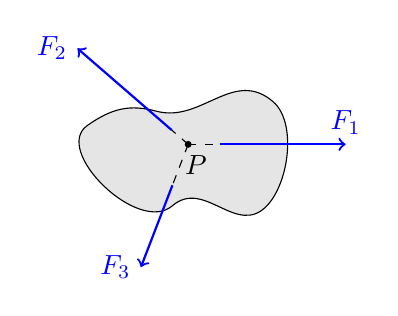
\begin{tikzpicture}[xscale=0.4, yscale=0.6]
	\draw[fill=gray!20] (-3.2,0.4) to [out=25,in=170] (-1,0.7) to [out=-10,in=150] (2.7,0.9) to [out=-30,in=35] (2.5,-1.3) to [out=215,in=30] (-0.5,-1.3) to [out=210,in=205] (-3.2,0.4);
	\draw[thick, blue, ->] (1,0) --++ (4,0) node[above]{$F_1$};
	\draw[thick, blue, ->] (240:1) --++ (240:2) node[left]{$F_3$};
	\draw[thick, blue, ->] (150:0.6) --++ (150:3.46) node[left]{$F_2$};
	\draw[dashed] (0,0) -- (1,0);
	\draw[dashed] (0,0) -- (240:1);
	\draw[dashed] (0,0) -- (150:0.6);
	\draw[fill] (0,0) circle(0.09 and 0.06);
	\node at (-60:0.5) {$P$};
	\end{tikzpicture}
	\vspace*{-15pt}
\end{marginfigure}

Suppose lines of action of $F_1$ and $F_2$ meet at point $P$, the moment of $F_1$ and moment of $F_2$ about $P$ are both zero. To produce zero resultant moment about $P$, then moment of $F_3$ about $P$ must vanish which suggests that the line of action of $F_3$ must pass through point $P$.
The lines of action of $F_1$, $F_2$ and $F_3$ therefore, must pass through the same point\footnote{In the case of three parallel forces in equilibrium, we can introduce the notion of an ideal point at infinity, so that parallel lines could meet at that point(!).}

Such three forces are said to be \emph{concurrent}

\subsection*{Summary for three forces in equilibrium}

For three forces in equilibrium, we can now conclude:

\begin{compactenum}
	\item[--] the three force vectors must be able to form a force triangle
	
	this is a consequence of zero resultant force
	
	\item[--] the lines of action for the three forces must pass through same point
	
	this is a consequence of zero resultant moment
\end{compactenum}






\subsection{End-of-chapter questions}


\subsection*{Mechanical equilibrium}

\question{Is it possible for an object to be in equilibrium if only one force is acting on it?}

\question{If three forces are in equilibrium, suggest and explain whether the lines of action must lie in the same plane.}
